\documentclass[tikz,border=10pt]{standalone}
\usepackage{tikz}
\usetikzlibrary{decorations.pathmorphing, arrows.meta}

\begin{document}
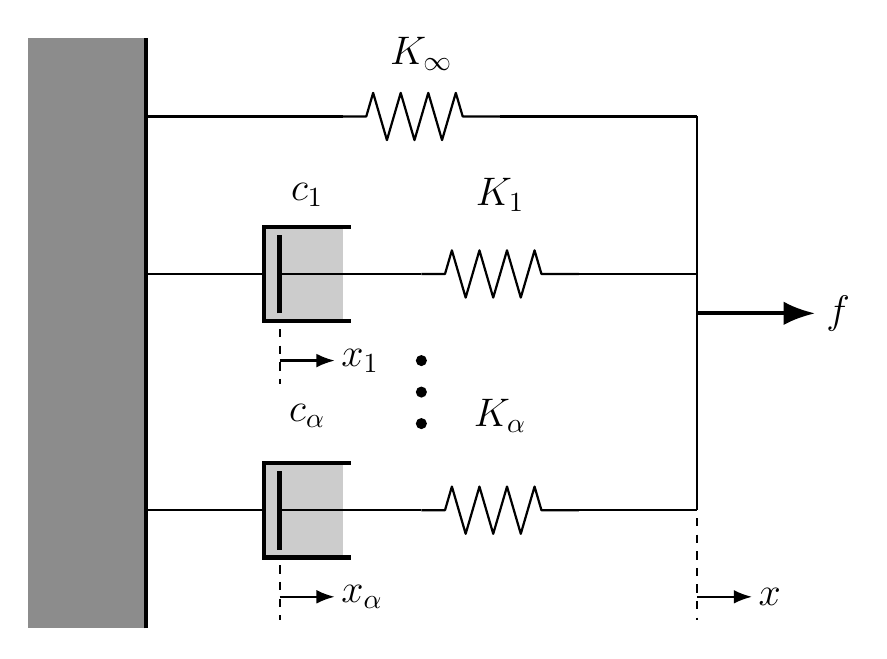
\begin{tikzpicture}[
    spring/.style={thick, decorate, decoration={zigzag, pre length=0.3cm, post length=0.3cm, segment length=3.5mm, amplitude=3mm}, line join=round},
    dashpot_cup/.style={line width=1.5pt},
    piston/.style={line width=2pt},
    wall/.style={fill=gray!90},
    wall_line/.style={ultra thick}
]

% --- Pared Izquierda ---
\fill[wall] (-1.5, -3.5) rectangle (0, 4);
\draw[wall_line] (0, -3.5) -- (0, 4);

% --- Rama Superior (Muelle infinito) ---
\draw[thick] (0, 3) -- (2.5, 3);
\draw[spring] (2.5, 3) -- (4.5, 3);
\draw[thick] (4.5, 3) -- (7, 3);
\node at (3.5, 3.8) {\Large $K_\infty$};

% --- Rama Intermedia 1 (Amortiguador y Muelle 1) ---
\fill[lightgray!80] (1.5, 0.4) rectangle (2.5, 1.6);
\draw[dashpot_cup] (2.6, 1.6) -- (1.5, 1.6) -- (1.5, 0.4) -- (2.6, 0.4);
\draw[thick] (0, 1) -- (1.5, 1);
\draw[piston] (1.7, 0.5) -- (1.7, 1.5);
\draw[thick] (1.7, 1) -- (3.5, 1);
\draw[spring] (3.5, 1) -- (5.5, 1);
\draw[thick] (5.5, 1) -- (7, 1);

% Etiquetas de la Rama 1
\node at (2.05, 2.0) {\Large $c_1$};
\node at (4.5, 2.0) {\Large $K_1$};

% Flecha de desplazamiento x1
\draw[thick, dashed] (1.7, 0.3) -- (1.7, -0.4);
\draw[thick, -Latex] (1.7, -0.1) -- (2.4, -0.1) node[right, inner sep=2pt] {\Large $x_1$};

% --- Puntos suspensivos ---
\fill (3.5, -0.1) circle (2pt);
\fill (3.5, -0.5) circle (2pt);
\fill (3.5, -0.9) circle (2pt);

% --- Rama Inferior (Amortiguador y Muelle alpha) ---
\fill[lightgray!80] (1.5, -2.6) rectangle (2.5, -1.4);
\draw[dashpot_cup] (2.6, -1.4) -- (1.5, -1.4) -- (1.5, -2.6) -- (2.6, -2.6);
\draw[thick] (0, -2) -- (1.5, -2);
\draw[piston] (1.7, -2.5) -- (1.7, -1.5);
\draw[thick] (1.7, -2) -- (3.5, -2);
\draw[spring] (3.5, -2) -- (5.5, -2);
\draw[thick] (5.5, -2) -- (7, -2);

% Etiquetas de la Rama alpha
\node at (2.05, -0.8) {\Large $c_\alpha$};
\node at (4.5, -0.8) {\Large $K_\alpha$};

% Flecha de desplazamiento x_alpha
\draw[thick, dashed] (1.7, -2.7) -- (1.7, -3.4);
\draw[thick, -Latex] (1.7, -3.1) -- (2.4, -3.1) node[right, inner sep=2pt] {\Large $x_\alpha$};

% --- Conexiones de la Derecha y Fuerza Aplicada ---
% Línea vertical común
\draw[thick] (7, 3) -- (7, -2);

% Vector de Fuerza f
\draw[line width=1.5pt, -{Latex[length=4mm, width=3mm]}] (7, 0.5) -- (8.5, 0.5) node[right] {\Large $f$};

% Flecha de desplazamiento total x
\draw[thick, dashed] (7, -2.1) -- (7, -3.4);
\draw[thick, -Latex] (7, -3.1) -- (7.7, -3.1) node[right, inner sep=2pt] {\Large $x$};

\end{tikzpicture}
\end{document}